% https://tex.stackexchange.com/a/471747
\documentclass{beamer}

\usepackage{tikz}
\usetikzlibrary{positioning}

\begin{document}

\begin{frame}{}

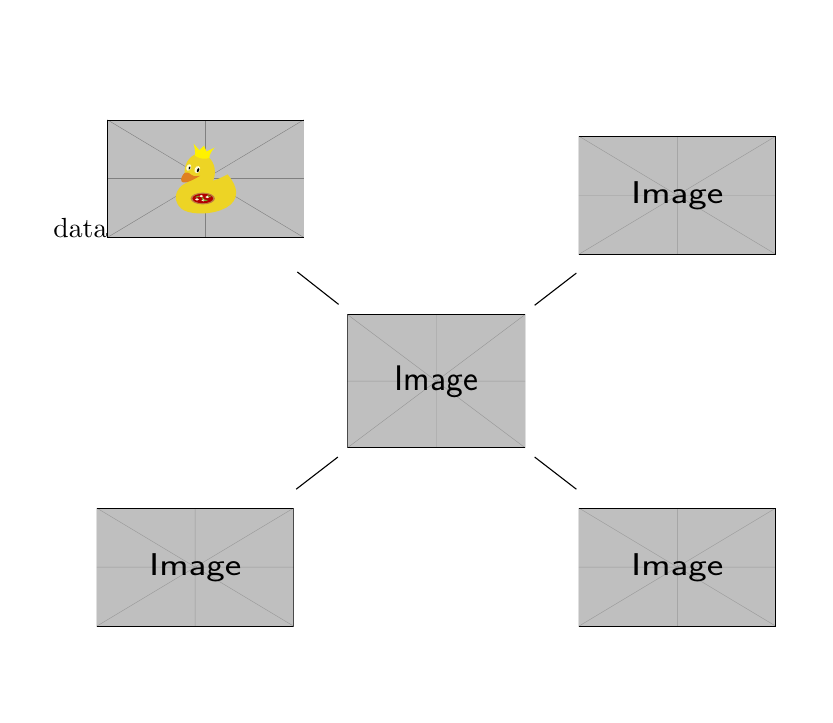
\begin{tikzpicture}[
            scale = 1.0, % <-- modify this number for scaling up/down
            invisi/.style  = {circle, draw = white, minimum size = 5mm},
        ]
        \node[invisi] (0)  {\includegraphics[scale=0.2]{example-image}};
        \node[invisi] (1) [above left= 0.1 cm and 0.8 cm of 0 ]{\hyperlink{data}{\includegraphics[width=2.5cm, height=1.5cm]{example-image-duck}}};
        \node[invisi] (2) [above right=0.1 cm and 0.8 cm of 0] {\includegraphics[width=2.5cm, height=1.5cm]{example-image}};
        \node[invisi] (3) [below left= 0.1 cm and 0.8 cm of 0]  {\includegraphics[width=2.5cm, height=1.5cm]{example-image}};
        \node[invisi] (4) [below right= 0.1 cm and 0.8 cm of 0]  {\includegraphics[width=2.5cm, height=1.5cm]{example-image}};

             \draw (0) -- (1);
             \draw (0) -- (2);
             \draw (0) -- (3);
             \draw (0) -- (4);
    \end{tikzpicture}


\end{frame}


\begin{frame}[label=data]

The data is presented here

\end{frame}

\end{document}
